
\Problem{L'amenaça fractal}

\Statement

L'amenaça fractal ens porta cap aquest destí:

\begin{center}
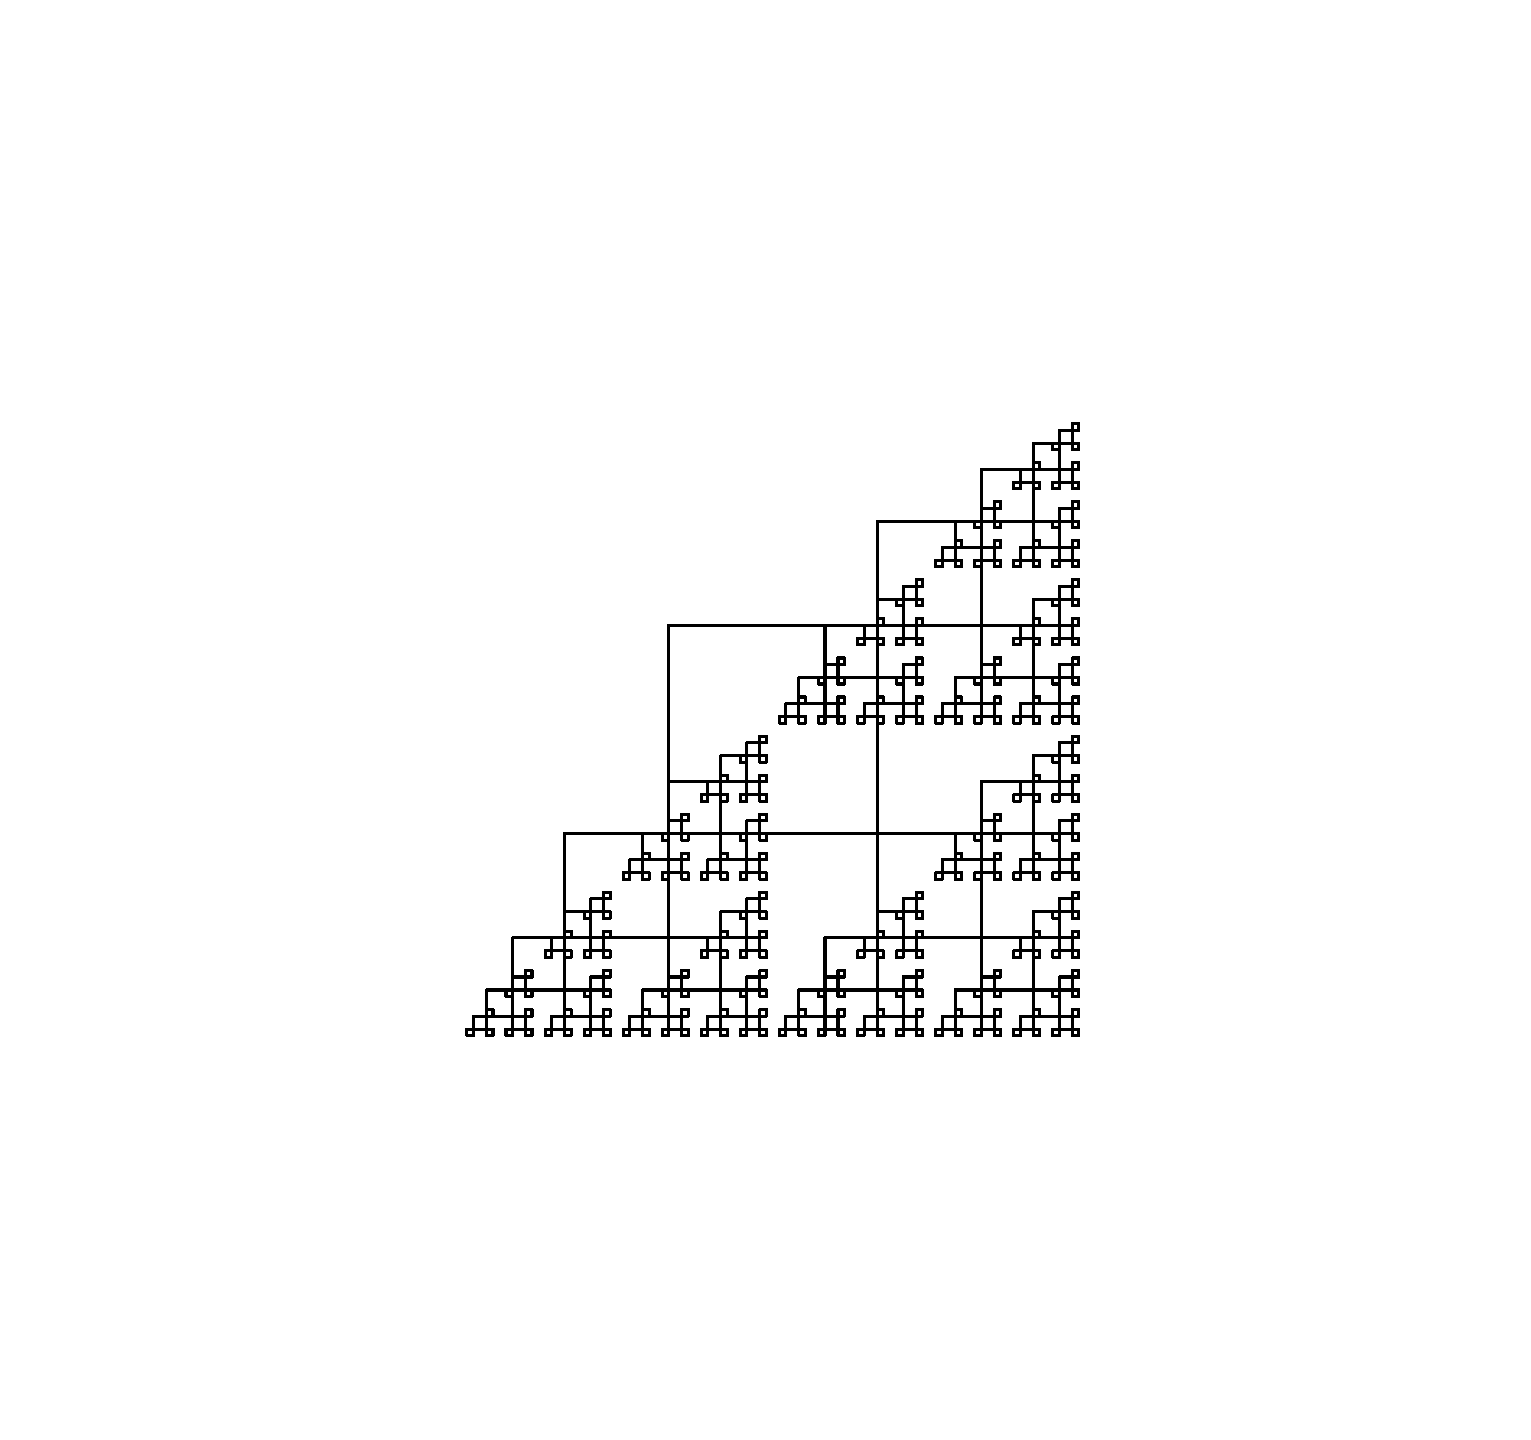
\includegraphics[trim=500 500 500 500,height=10cm]{6.eps}
\end{center}

Per pintar una amenaça fractal de $n\ge1$ nivells de mida $d$, cal pintar un quadrat
de mida~$d$, i tres amenaces fractals a tres de les seves quatre cantonades
amb $n-1$ nivells i mida $d/2$. Una amenaça fractal de zero nivells és buida.
\bigskip

Per exemple, aquestes són les amenaces fractals amb 1, 2, 3, 4, 5 i 6 nivells:

\begin{center}
1 ~
\fbox{

\includegraphics[trim=500 500 500 500,height=3.5cm]{1.eps}
}
\qquad
2 ~
\fbox{
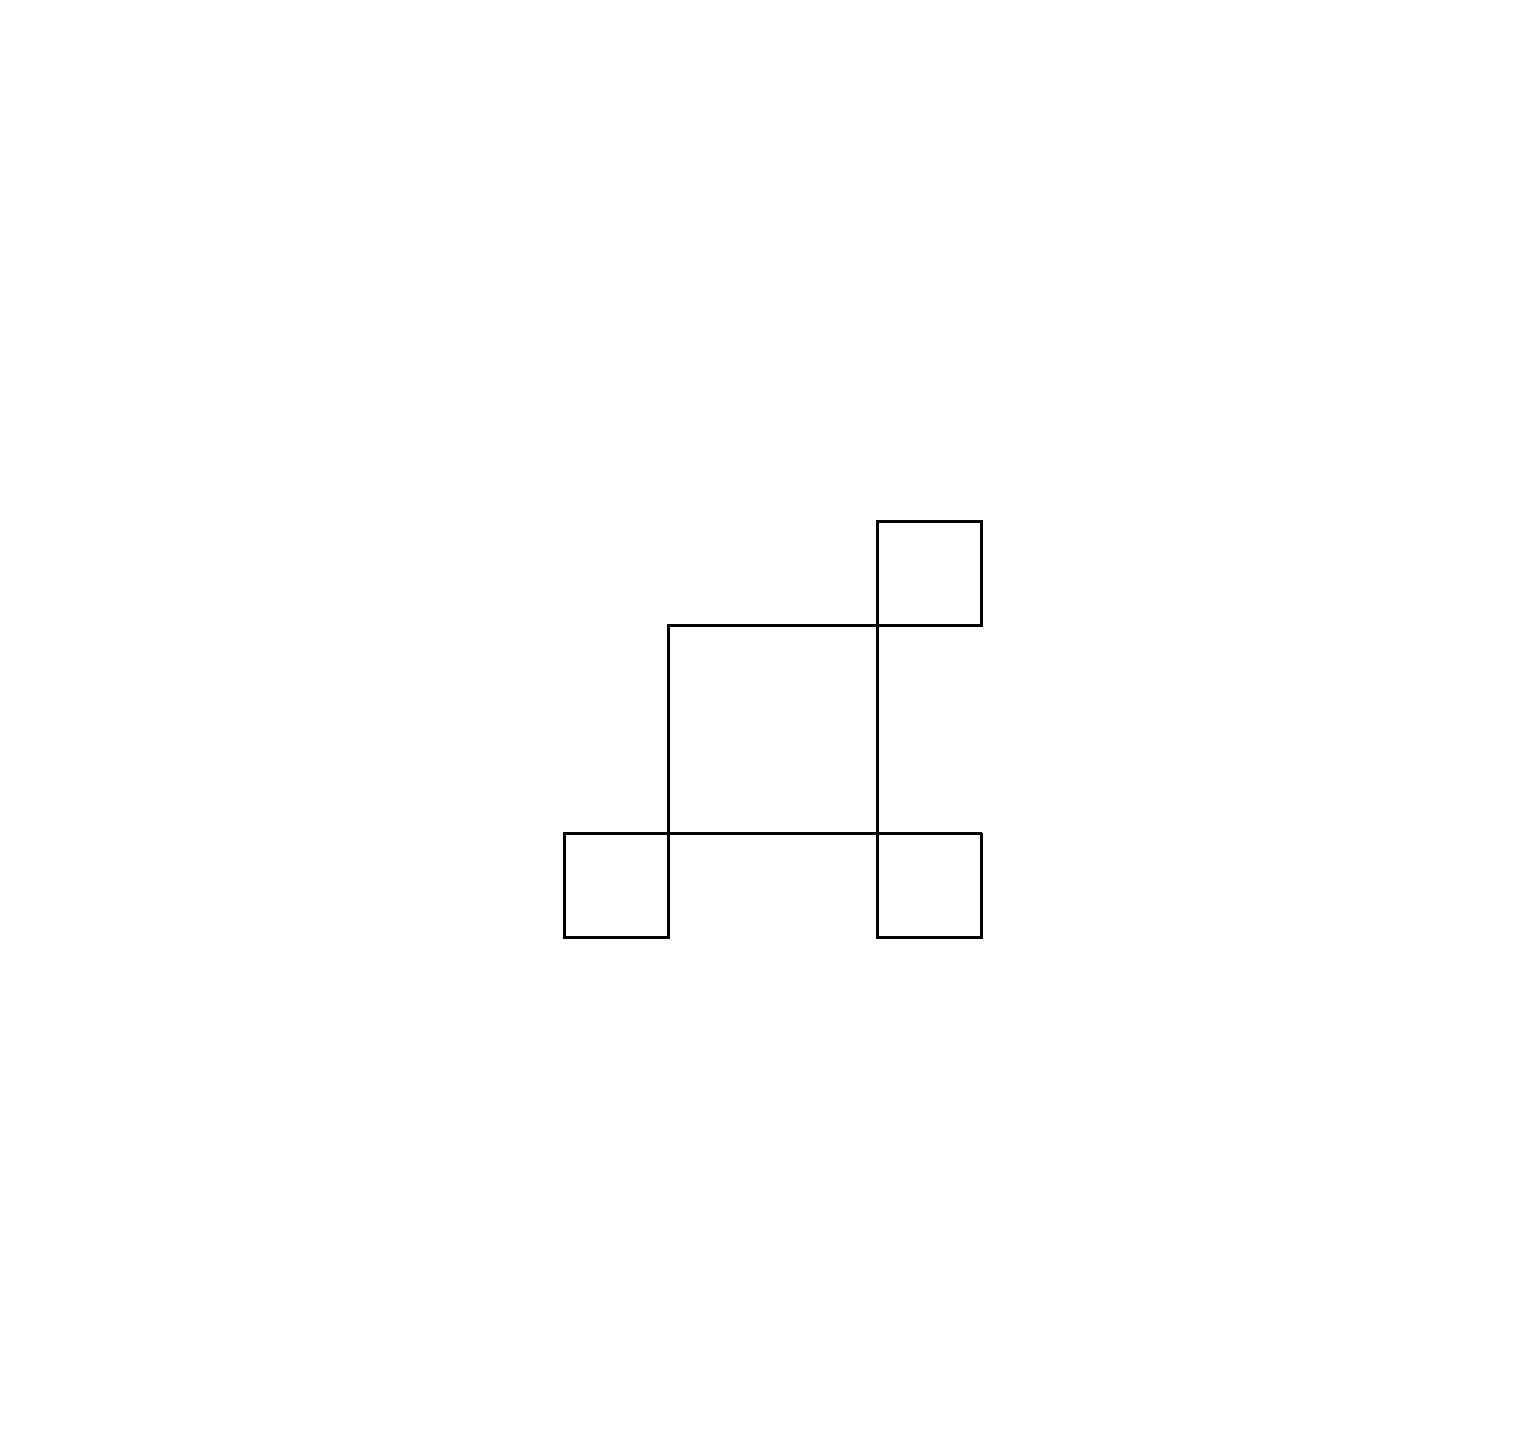
\includegraphics[trim=500 500 500 500,height=3.5cm]{2.eps}
}
\qquad
3 ~
\fbox{
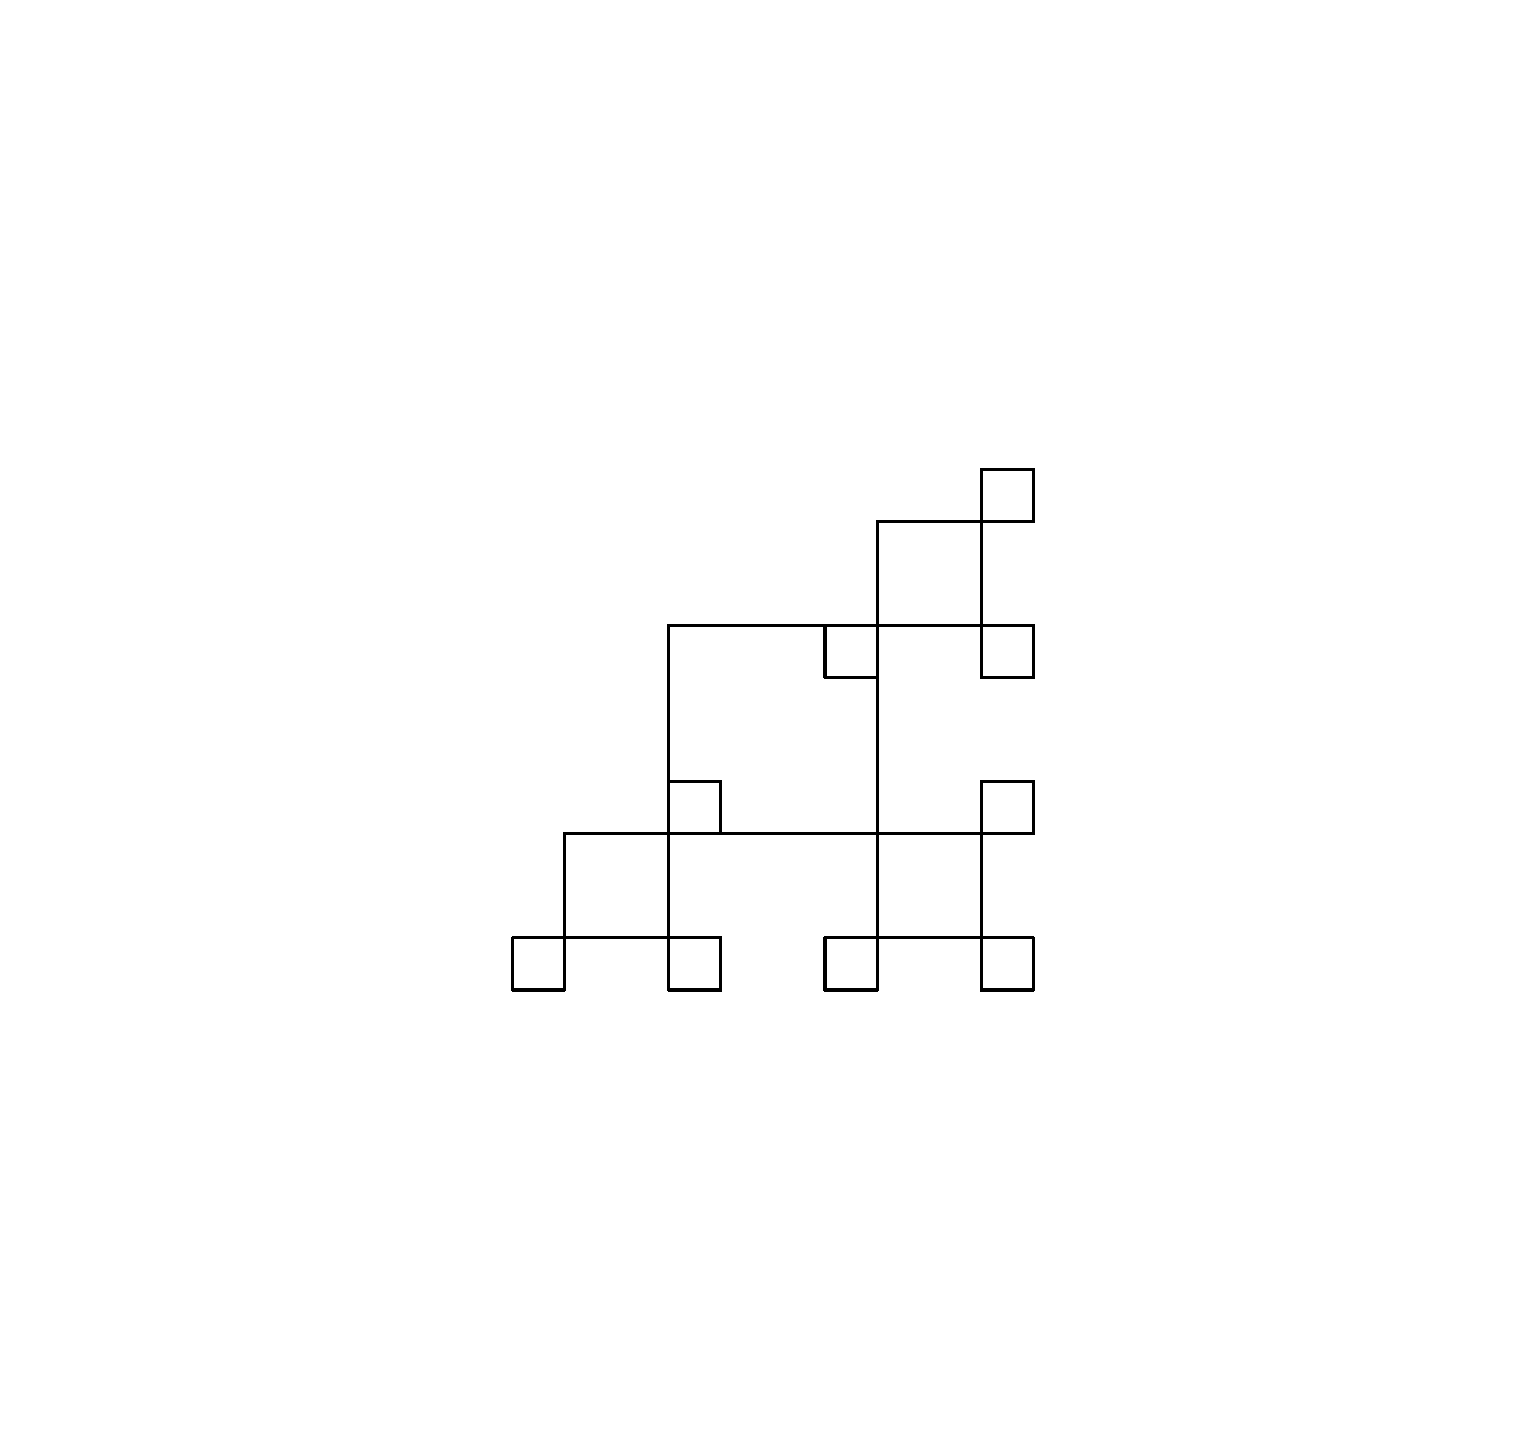
\includegraphics[trim=500 500 500 500,height=3.5cm]{3.eps}
}

\bigskip
\bigskip

4 ~
\fbox{
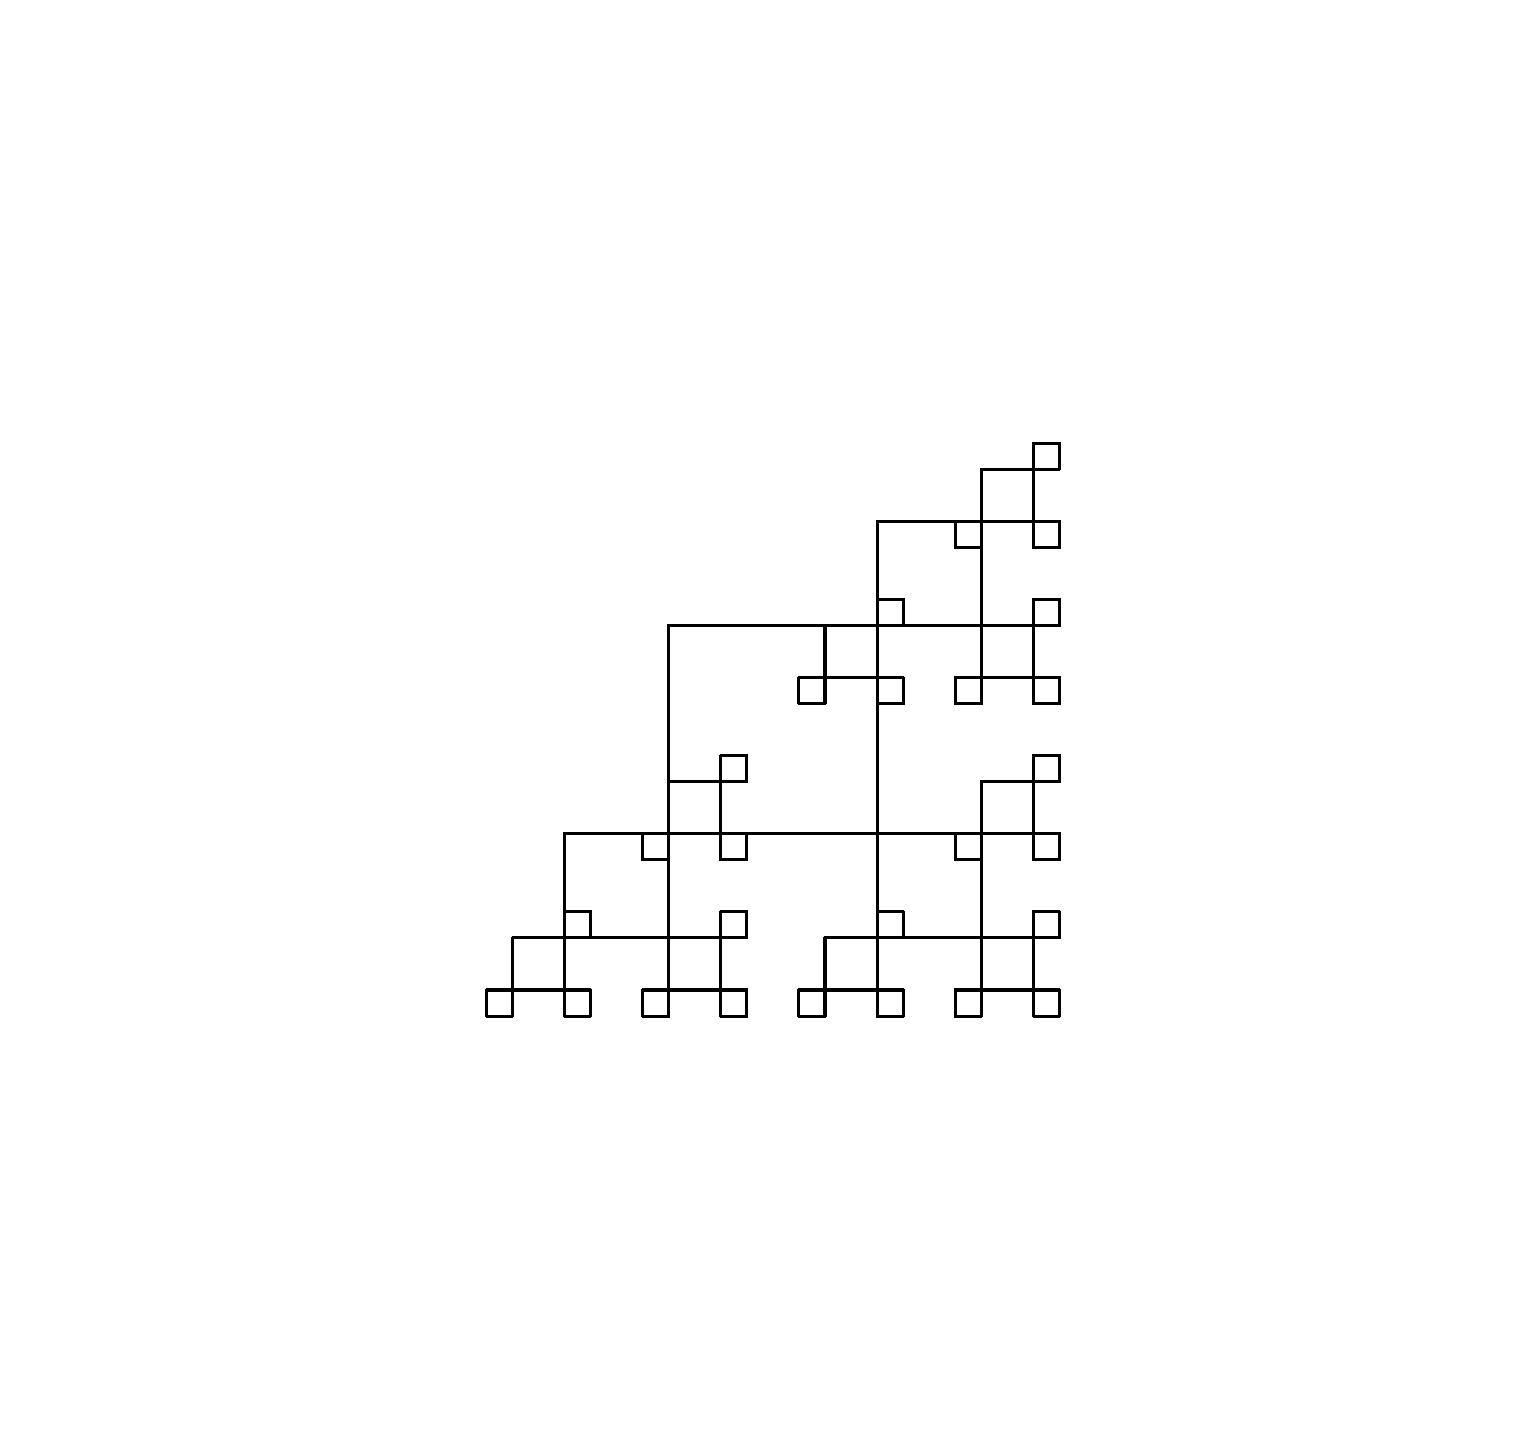
\includegraphics[trim=500 500 500 500,height=3.5cm]{4.eps}
}
\qquad
5 ~
\fbox{
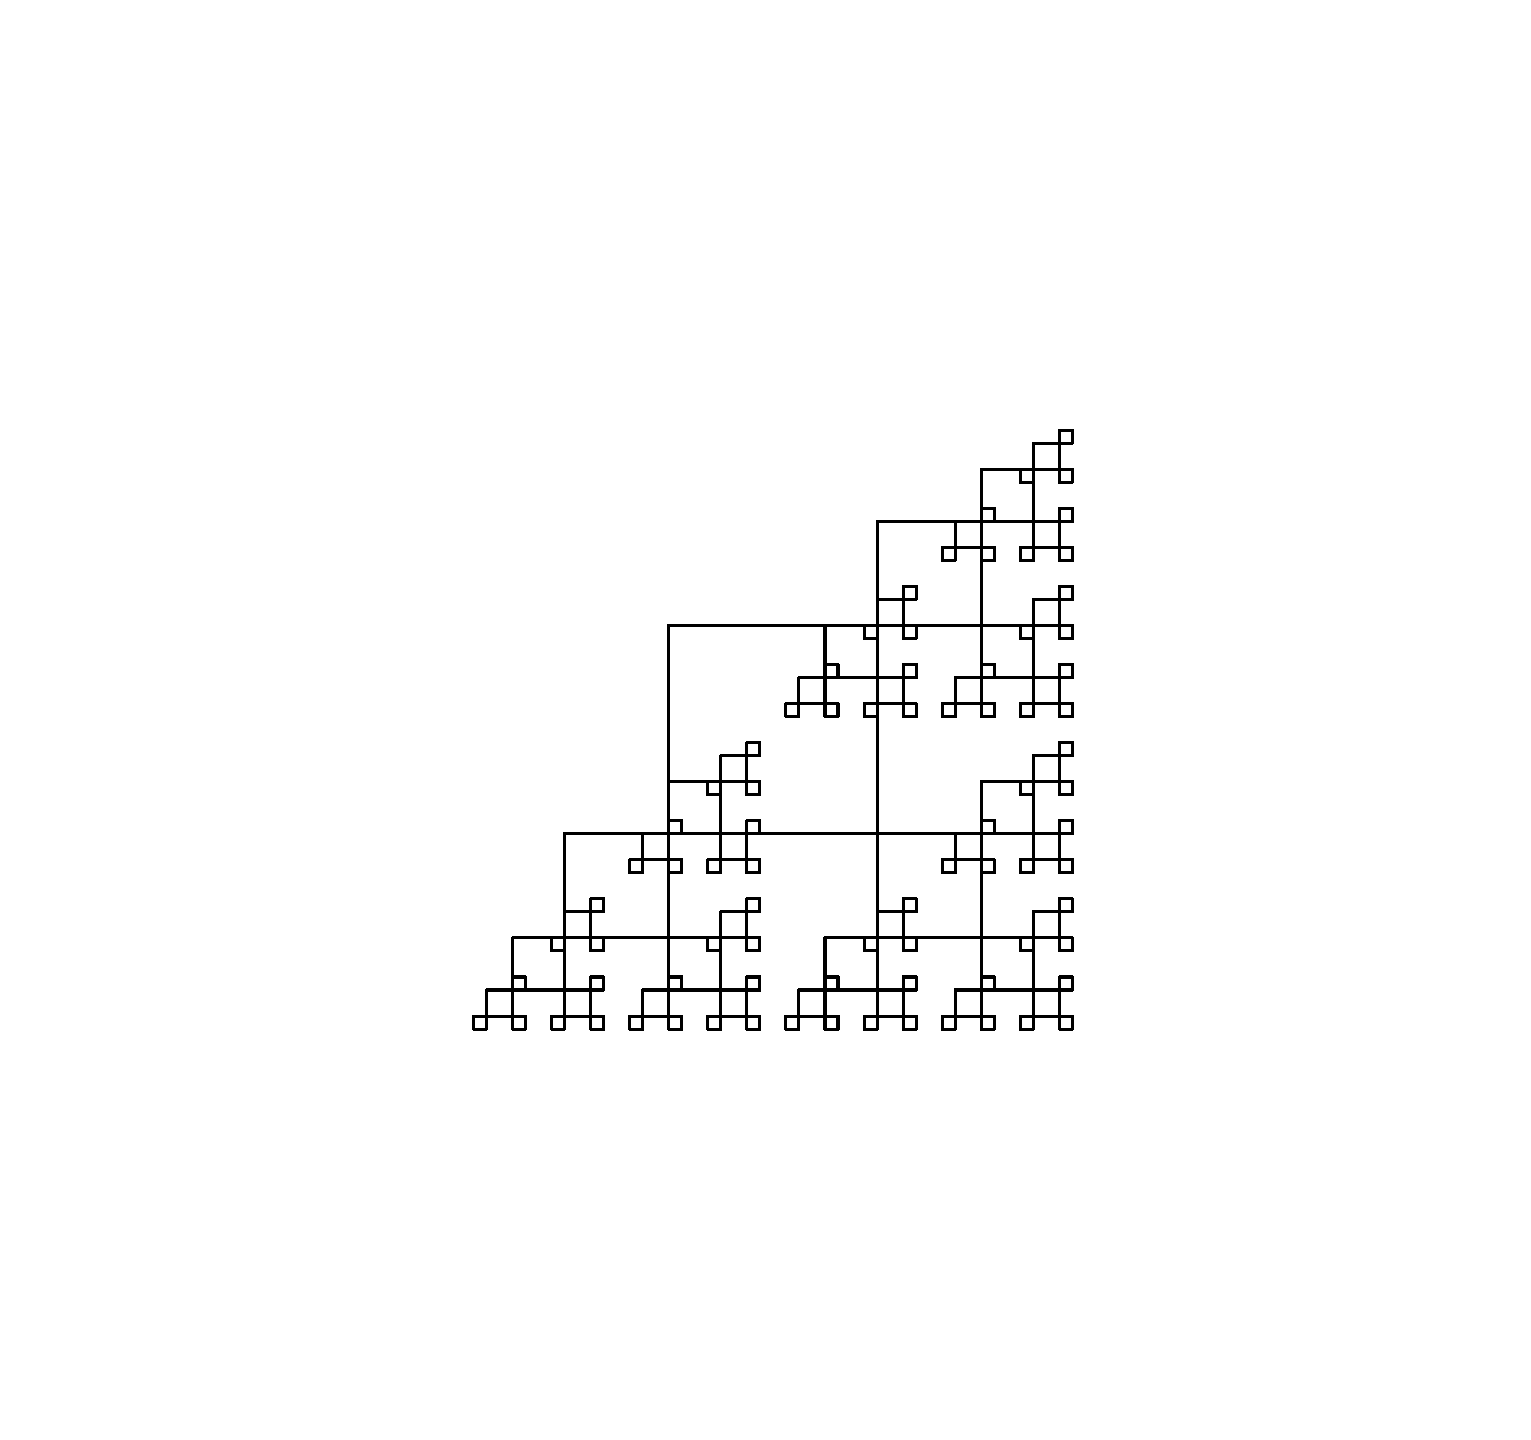
\includegraphics[trim=500 500 500 500,height=3.5cm]{5.eps}
}
\qquad
6 ~
\fbox{
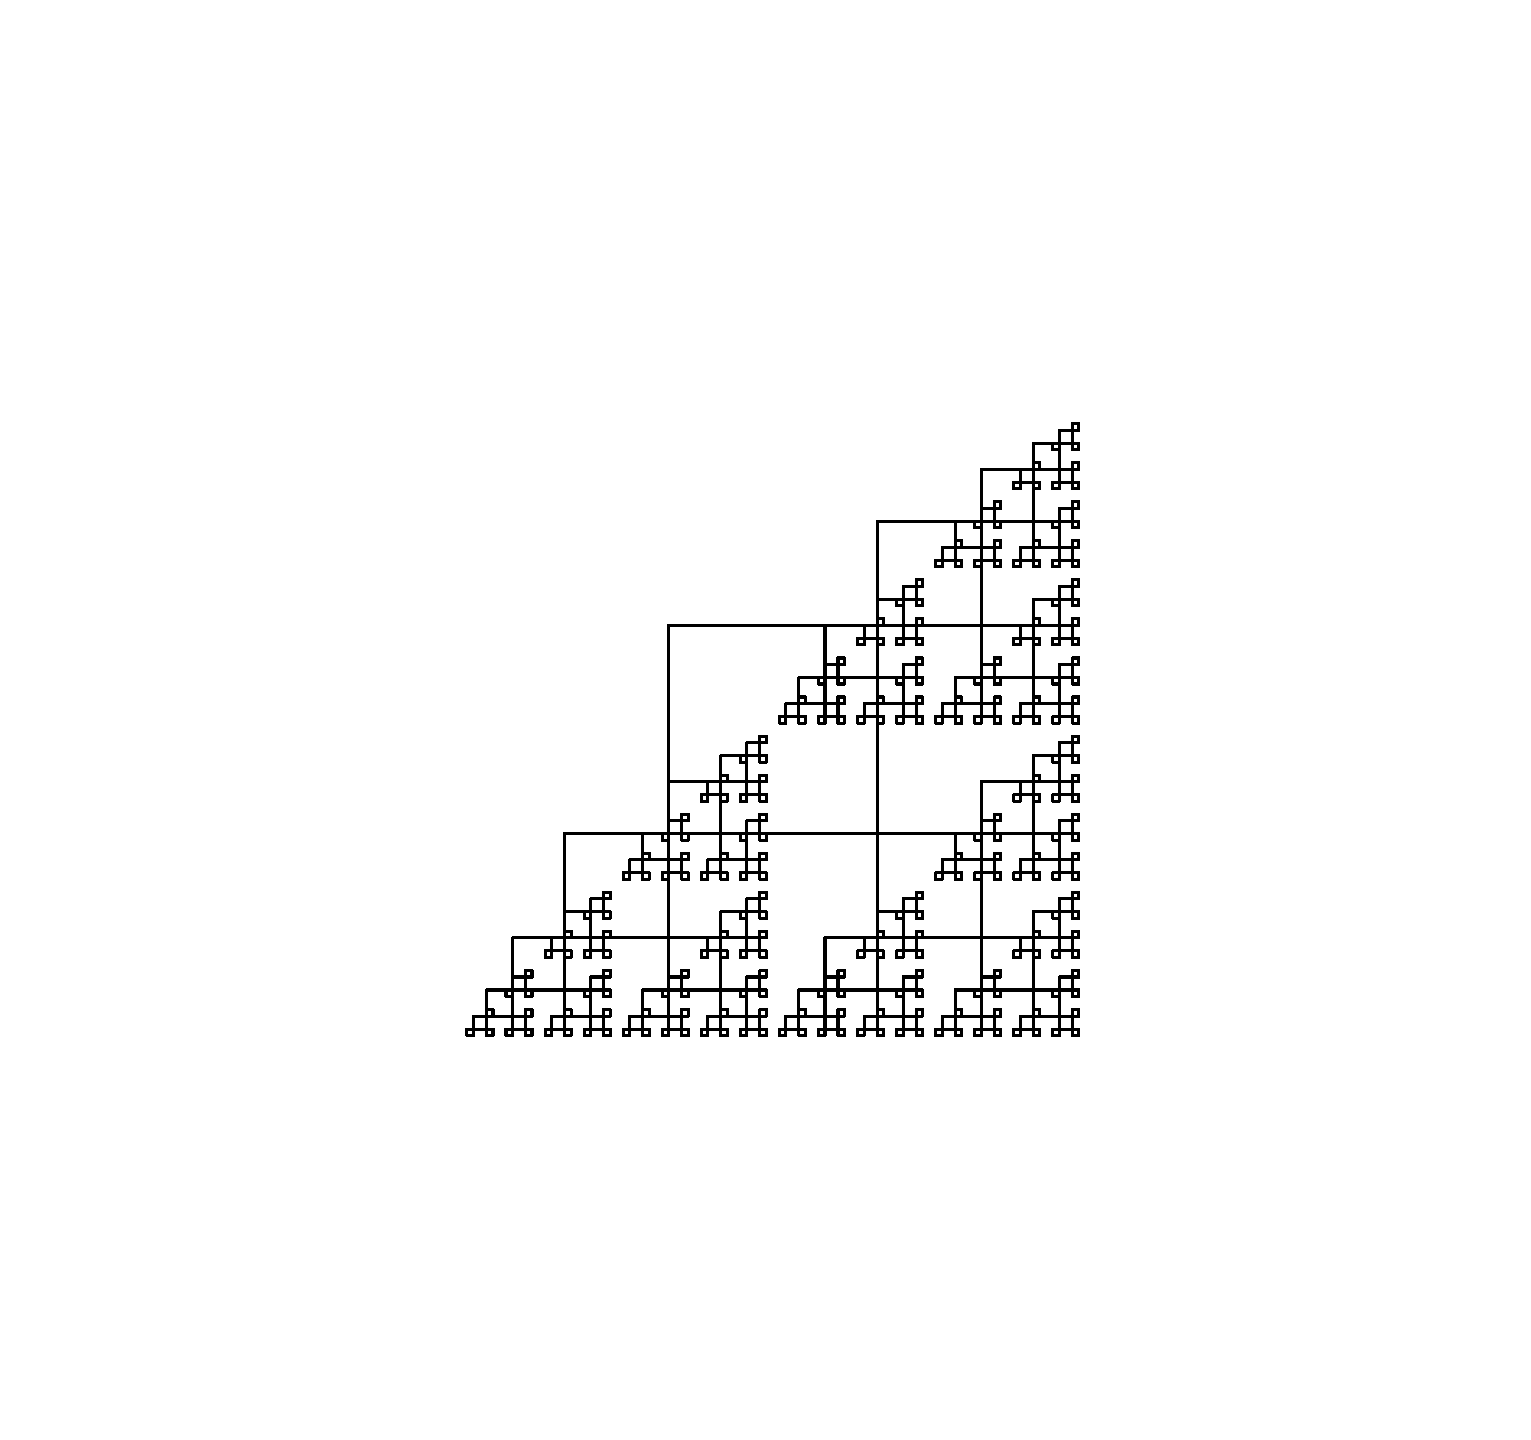
\includegraphics[trim=500 500 500 500,height=3.5cm]{6.eps}
}
\end{center}

\mysection{Entrada}

A l'entrada, es dónen dos valors: un natural $n$ amb el nombre de nivells del
fractal i un real positiu $d$ amb la seva mida.

\mysection{Sortida}

El programa ha de dibuixar l'amenaça fractal d'$n$ nivells i
mida $d$ centrat a la finestra.

\bigskip

\begin{multicols}{2}\raggedcolumns
\mysection{Exemple d'entrada 1}

\begin{verbatim}
4
100
\end{verbatim}

\columnbreak

\mysection{Exemple de sortida 1}

\fbox{

\includegraphics[trim=500 500 500 500,height=3.5cm]{sample1.eps}
}

\end{multicols}

\begin{multicols}{2}\raggedcolumns
\mysection{Exemple d'entrada 2}

\begin{verbatim}
2
50
\end{verbatim}


\columnbreak
\mysection{Exemple de sortida 2}

\fbox{
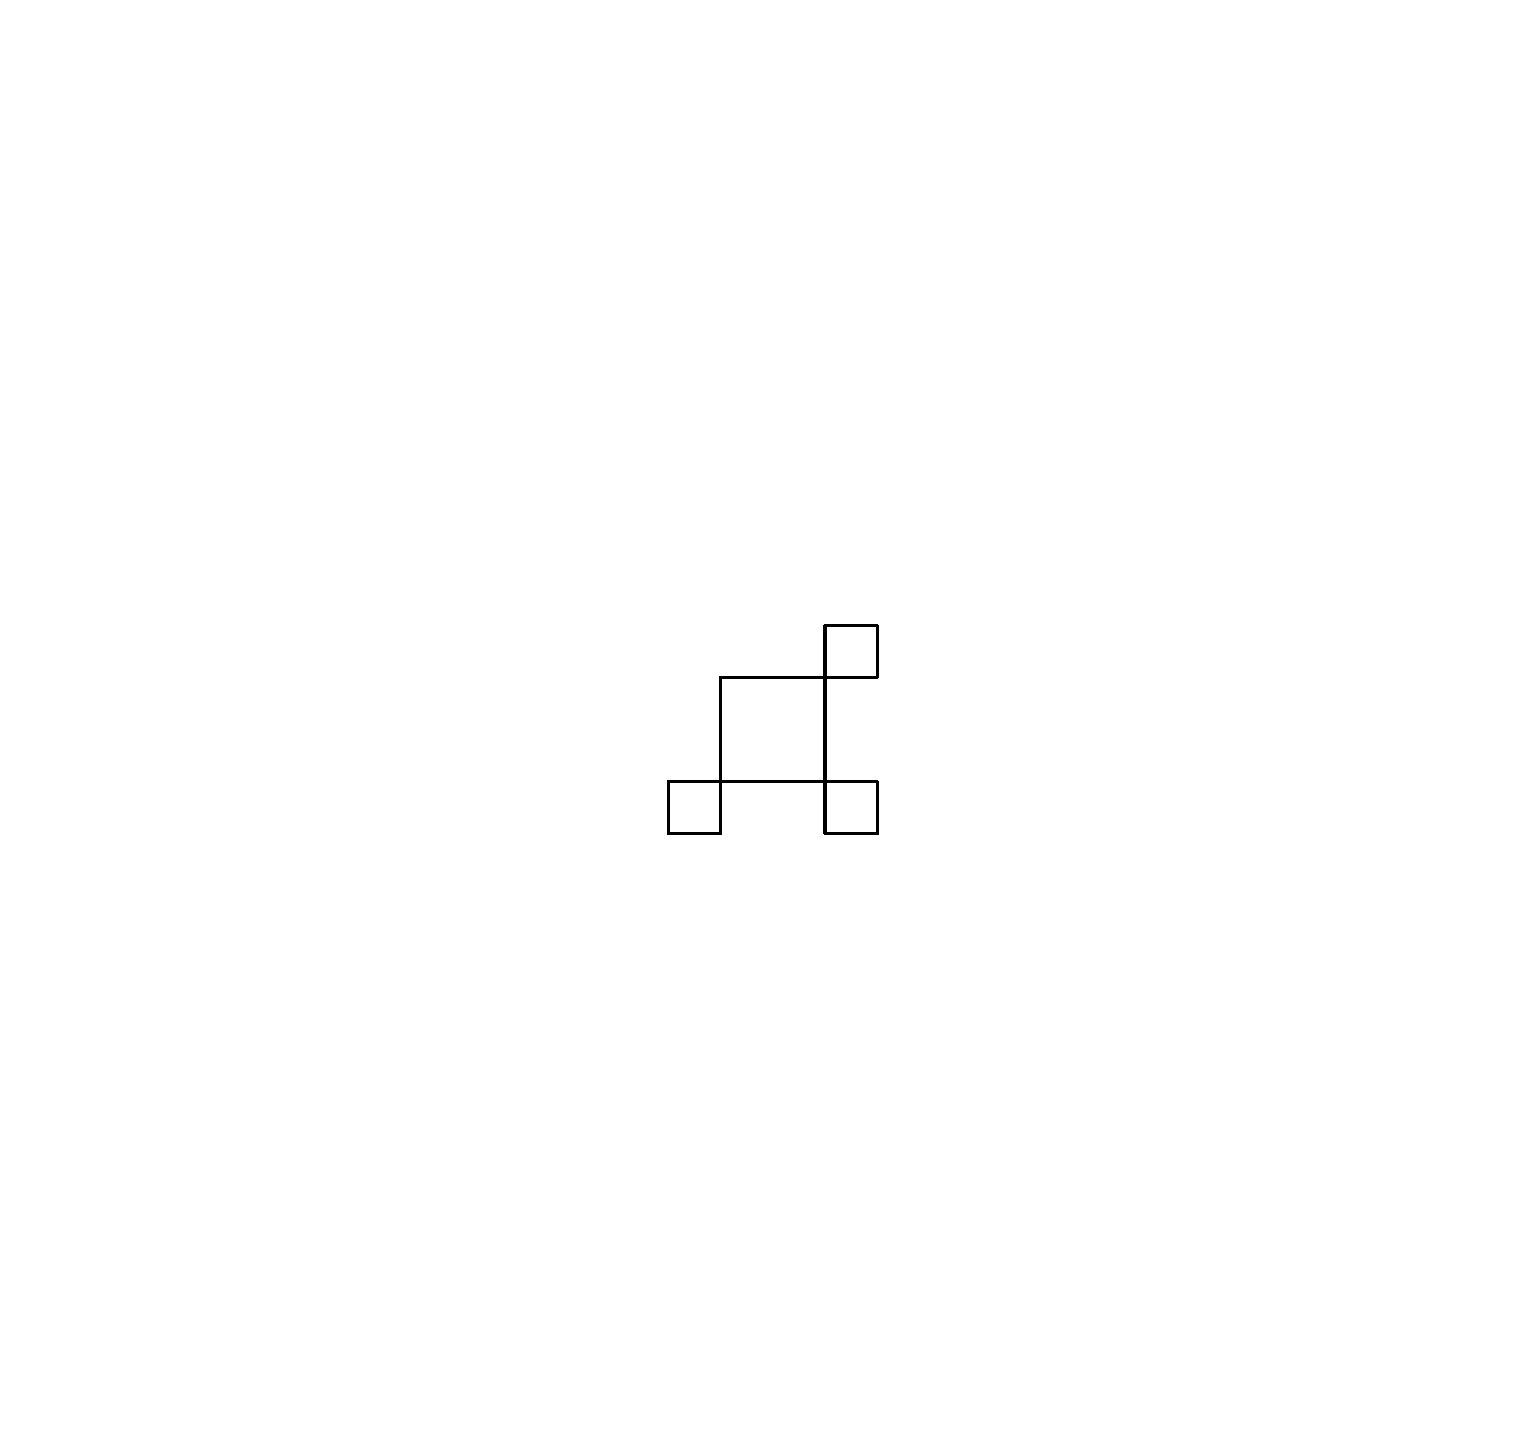
\includegraphics[trim=500 500 500 500,height=3.5cm]{sample2.eps}
}

\end{multicols}


\mysection{Recordatori}

Recordeu que Python ofereix un mòdul \texttt{turtle} que permet pintar images.
Les úniques operacions que us calen són
\texttt{turtle.goto(x, y)} que mou la tortuga a les coordenades (\texttt{x},\texttt{y}),
\texttt{turtle.forward(d)} que avança la tortuga \texttt{d} unitats,
\texttt{turtle.left(a)} que gira la tortuga \texttt{a} graus cap a l'esquerra,
\texttt{turtle.down()} que activa el traçat i
\texttt{turtle.up()} que desactiva el traçat.


\mysection{Important}

Aquest problema no té jocs de proves al Jutge. Per tant, qualsevol solució serà
acceptada: semàfor verd! Això no vol dir que sigui bona ni dolenta, el vostre
professor ho corregirà.
